%%%%%%%%%%%%%%%%%%%%%%%%%%%%%%%%%%%%%%%%%%%%%%%%%%%%%%%%%%%%%%%
%
% Welcome to writeLaTeX --- just edit your LaTeX on the left,
% and we'll compile it for you on the right. If you give
% someone the link to this page, they can edit at the same
% time. See the help menu above for more info. Enjoy!
%
%%%%%%%%%%%%%%%%%%%%%%%%%%%%%%%%%%%%%%%%%%%%%%%%%%%%%%%%%%%%%%%

% --------------------------------------------------------------
% This is all preamble stuff that you don't have to worry about.
% Head down to where it says "Start here"
% --------------------------------------------------------------
 
\documentclass[12pt]{article}
 
\usepackage[margin=1in]{geometry}
\usepackage{amsmath,amsthm,amssymb}
\usepackage{enumitem}
\usepackage{cancel}

\setlist[enumerate,1]{label={(\alph*)}} %this changes enumerate to (a),(b),...

\usepackage{graphicx} %package to manage images

\newcommand{\A}{{\mathcal{A}}}
\newcommand{\C}{{\mathbb C}}
\newcommand{\CC}{{\mathcal{C}}}
\newcommand{\N}{{\mathbb N}}
\newcommand{\R}{{\mathbb R}}
\newcommand{\Q}{{\mathbb Q}}
\newcommand{\Z}{{\mathbb Z}}

\newcommand{\Aut}{{\rm Aut}}
\newcommand{\End}{{\rm End}}
\newcommand{\Hom}{{\rm Hom}}
\newcommand{\id}{{\rm id}}
\newcommand{\Ima}{{\rm Im}}
\newcommand{\Ker}{{\rm Ker}}
\newcommand{\Mor}{{\rm Mor}}
\newcommand{\Rad}{{\rm Rad}}
\newcommand{\Prob}{{\sf P}}
\newcommand{\E}{{\sf E}}
\newcommand{\Var}{{\sf Var}}

\renewcommand\labelitemi{-} %this changes itemize bullet points to dashes (-)

\usepackage{listings}
\usepackage{xcolor}

%New colors defined below
\definecolor{codegreen}{rgb}{0,0.6,0}
\definecolor{codegray}{rgb}{0.5,0.5,0.5}
\definecolor{codepurple}{rgb}{0.58,0,0.82}
\definecolor{backcolour}{rgb}{0.95,0.95,0.92}

%Code listing style named "mystyle"
\lstdefinestyle{mystyle}{
  backgroundcolor=\color{backcolour}, commentstyle=\color{codegreen},
  keywordstyle=\color{magenta},
  numberstyle=\tiny\color{codegray},
  stringstyle=\color{codepurple},
  basicstyle=\ttfamily\footnotesize,
  breakatwhitespace=false,         
  breaklines=true,                 
  captionpos=b,                    
  keepspaces=true,                 
  numbers=left,                    
  numbersep=5pt,                  
  showspaces=false,                
  showstringspaces=false,
  showtabs=false,                  
  tabsize=2
}

%"mystyle" code listing set
\lstset{style=mystyle}
 
\newenvironment{theorem}[2][Theorem]{\begin{trivlist}
\item[\hskip \labelsep {\bfseries #1}\hskip \labelsep {\bfseries #2.}]}
{\end{trivlist}}
\newenvironment{lemma}[2][Lemma]{\begin{trivlist}
\item[\hskip \labelsep {\bfseries #1}\hskip \labelsep {\bfseries #2.}]}
{\end{trivlist}}
\newenvironment{exercise}[2][Exercise]{\begin{trivlist}
\item[\hskip \labelsep {\bfseries #1}\hskip \labelsep {\bfseries #2.}]}
{\end{trivlist}}
\newenvironment{problem}[2][Problem]{\begin{trivlist}
\item[\hskip \labelsep {\bfseries #1}\hskip \labelsep {\bfseries #2.}]}
{\end{trivlist}}
\newenvironment{question}[2][Question]{\begin{trivlist}
\item[\hskip \labelsep {\bfseries #1}\hskip \labelsep {\bfseries #2.}]}
{\end{trivlist}}
\newenvironment{corollary}[2][Corollary]{\begin{trivlist}
\item[\hskip \labelsep {\bfseries #1}\hskip \labelsep {\bfseries #2.}]}
{\end{trivlist}}

\newenvironment{solution}{\begin{proof}[Solution]}{\end{proof}}
 
\begin{document}
 
% --------------------------------------------------------------
%                         Start here
% --------------------------------------------------------------
 
\title{Homework 6}%replace X with the appropriate number
\author{Mengxiang Jiang\\ %replace with your name
Stat 610 Distribution Theory} %if necessary, replace with your course title
 
\maketitle

\begin{problem}{1}
  Let $X$ have the \textit{Laplace} distribution (recalling Problem 3 
  of Assignment 4), with pdf
  \[
    f(x) = \frac{\lambda}{2} e^{-\lambda |x|}, \quad \text{all } x.
  \]
  Now suppose $a > 0$ and $b \in (-\infty, \infty)$. Let $Y = aX + b$.
  \begin{enumerate}
    \item Find the pdf for $Y$.
    \item Show that $X$ has mgf 
    $M_X(t) = \frac{1}{1 - \frac{t^2}{\lambda^2}}$. Hint: integrate
    two halves separately and then combine.
    \item Use the mgf and a property of mgfs (Theorem 2.28 in the notes)
    to obtain the mgf for $Y$.
  \end{enumerate}

  \begin{enumerate}
    \item Using the mnemonic
    \[
      f_Y(y) = f_X(x) \left| \frac{dx}{dy} \right|,
    \]
    where $x = \frac{y - b}{a}$, we have
    \[
      f_Y(y) = \frac{\lambda}{2a} e^{-\frac{\lambda}{a} |y - b|}, 
      \quad \text{all } y.
    \]
    \item The mgf of $X$ is 
    \[
      \begin{aligned}
        M_X(t) &= \E[e^{tX}] = \int_{-\infty}^{\infty} e^{tx} f(x) dx \\
        &= \int_{-\infty}^{0} e^{tx} \frac{\lambda}{2} e^{\lambda x} dx + 
        \int_{0}^{\infty} e^{tx} \frac{\lambda}{2} e^{-\lambda x} dx \\
        &= \frac{\lambda}{2} \int_{-\infty}^{0} e^{(t + \lambda)x} dx + 
        \frac{\lambda}{2} \int_{0}^{\infty} e^{(t - \lambda)x} dx \\
        &= \frac{\lambda}{2} \left[ \frac{1}{t + \lambda} 
        e^{(t + \lambda)x} \right]_{-\infty}^{0} + 
        \frac{\lambda}{2} \left[ \frac{1}{t - \lambda} 
        e^{(t - \lambda)x} \right]_{0}^{\infty} \\
        &= \frac{\lambda}{2} \left( \frac{1}{t + \lambda} - 
        \frac{1}{t - \lambda} \right) = \frac{1}{1 - \frac{t^2}{\lambda^2}},
      \end{aligned}
    \]
    \item \textbf{Theorem 2.28} Let $X$ have mgf $M_X$ and let $Y = aX + b$.\\
    Then $Y$ has mgf $M_Y(t) = e^{bt} M_X(at)$.
    \\\\
    Thus, the mgf of $Y$ is 
    \[
      M_Y(t) = e^{bt} M_X(at) = e^{bt} \frac{1}{1 - \frac{a^2 t^2}{\lambda^2}}.
    \]
  \end{enumerate}
\end{problem}

\begin{problem}{2}
  Determine the hazard functions for each of the following 
  (see Section 3.4 in the notes).
  \begin{enumerate}
    \item The gamma(2,$\beta$) distribution. (The cdf can be expressed
    explicitly in this case.) Use $\beta = 1,2,5$ for the plot (all together
    in one plot).
    \item The distribution with pdf $f(x) = \frac13 e^{-x} + \frac43 e^{-2x}$
    for $x > 0$. 
    [This is the so-called \textit{mixture} of two exponential pdfs.]
  \end{enumerate}
  \begin{enumerate}
    \item The pdf of gamma(2,$\beta$) distribution is
    \[
      f(x) = \frac{1}{\beta^2} x e^{-\frac{x}{\beta}}1_{(0,\infty)}(x).
    \]
    The cdf is
    \[
      F(x) = 1 - e^{-\frac{x}{\beta}} - \frac{x}{\beta} e^{-\frac{x}{\beta}}
      1_{(0,\infty)}(x).
    \]
    The hazard function is
    \[
      h(x) = \frac{f(x)}{1-F(x)} = \frac{\frac{1}{\beta^2} 
      x e^{-\frac{x}{\beta}}}{e^{-\frac{x}{\beta}} + 
      \frac{x}{\beta} e^{-\frac{x}{\beta}}} = 
      \frac{\frac{1}{\beta^2} x}{1 + \frac{x}{\beta}} = 
      \frac{x}{\beta(x + \beta)}.
    \]
    \begin{center}
      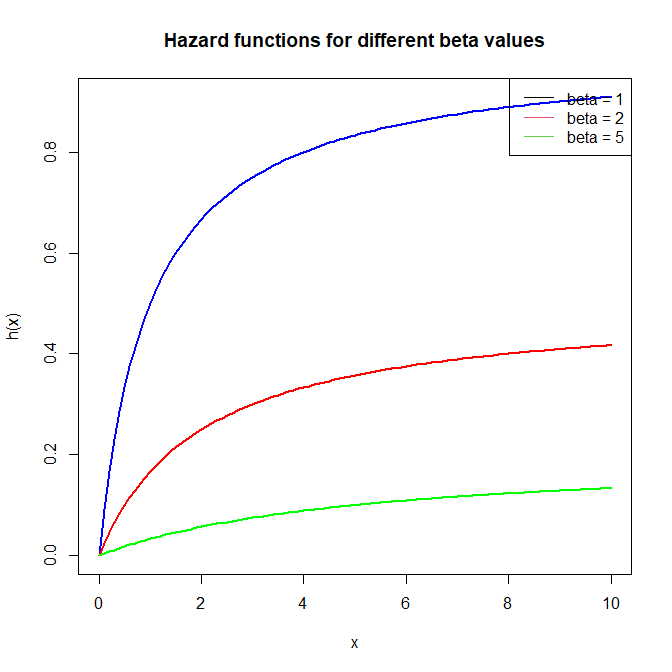
\includegraphics[width=0.8\textwidth]{2a.png}
    \end{center}
    \item The cdf is
    \[
      F(x) = \int_{0}^{x} \left( \frac13 e^{-t} + \frac43 e^{-2t} \right) dt 
      = \frac13 (1 - e^{-x}) + \frac23 (1 - e^{-2x}) = 1 - \frac13 e^{-x} - 
      \frac23 e^{-2x}.
    \]
    The hazard function is
    \[
      h(x) = \frac{f(x)}{1-F(x)} = \frac{\frac13 e^{-x} + \frac43 e^{-2x}}
      {\frac13 e^{-x} + \frac23 e^{-2x}} = \frac{1 + 4e^{-x}}{1 + 2e^{-x}}.
    \]
    \begin{center}
      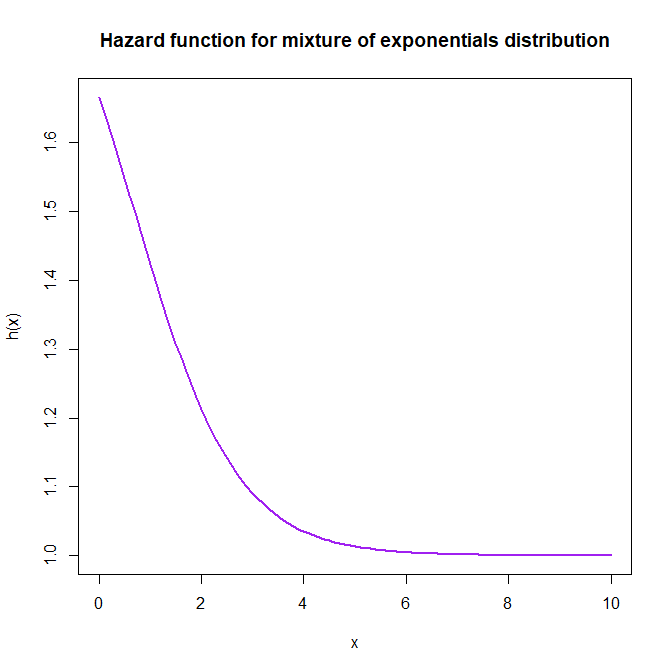
\includegraphics[width=0.8\textwidth]{2b.png}
    \end{center}
  \end{enumerate}
\end{problem}

\begin{problem}{3}
  Let $T$ be a positive random variable with hazard rate $h(t)$.
  \begin{enumerate}
    \item Find the quantile function for $T$ and identify 
    $\mathsf{med}(T)$ in terms of $H(t) = \int_0^t h(x)dx$.
    Apply to Weibull($\gamma$, $\beta$) which has cdf 
    $F_T(t) = 1 - e^{-t^{\gamma} / \beta}$ for $t \geq 0$.
    \item Consider the ``U-shaped" $h(t) = .5t^{-.5} + 6t^2$. 
    When is the failure rate at its lowest? Find
    the pdf.
  \end{enumerate}

  \begin{enumerate}
    \item We have
    \[
      \begin{aligned}
        H(t) &= \int_0^t h(x) dx\\
        &= \int_0^t \frac{f_T(x)}{1 - F_T(x)} dx \\
        &= -\int_0^t \frac{d(1 - F_T(x))}{1 - F_T(x)} \\
        &= -\left[ \ln(1 - F_T(x)) \right]_0^t \\ 
        &= -\ln(1 - F_T(t)) \\
        \Rightarrow F_T(t) &= 1 - e^{-H(t)}.
      \end{aligned}
    \]
    The quantile function is
    \[
      Q(p) = F_T^{-1}(p) = \left( -\ln(1 - p) \right)^{1/\gamma} \beta.
    \]
    The median is
    \[
      \mathsf{med}(T) = Q(0.5) = (\ln 2)^{1/\gamma} \beta.
    \]
    \item Since $h(t)$ is U-shaped, the failure rate is at its lowest 
    when $h'(t) = 0$.
    \[
      h'(t) = -0.25 t^{-1.5} + 12t = 0 \Rightarrow t = \left( \frac{1}{48} 
      \right)^{1/2} = \frac{1}{4\sqrt{3}}.
    \]
    The pdf is
    \[
      f(t) = h(t) e^{-H(t)} = \left( 0.5t^{-.5} + 6t^2 \right) e^{-H(t)},
    \]
    where
    \[
      H(t) = \int_0^t h(x) dx = \int_0^t \left( 0.5x^{-.5} + 6x^2 \right) dx 
      = t^{0.5} + 2t^3.
    \]
  \end{enumerate}
\end{problem}

\begin{problem}{4}
  Identify each of the following as defining a location family, 
  a scale family or a location-scale family (if any). 
  (Note: the given parameters are not necessarily location or scale.) 
  Determine the member of the family with mean = 0 (if location family), 
  variance = 1 (if scale family) or both (if location-scale family).
  \begin{enumerate}
    \item The uniform($a, b$) distributions.
    \item The Laplace distributions of Problem 1(a).
    \item The Weibull($\gamma$, $\beta$) distributions with $\gamma = 2$
    fixed.
  \end{enumerate}
  
  \begin{enumerate}
    \item The uniform($a, b$) distributions form a location-scale family,
    since if $X \sim \text{uniform}(0,1)$, then $Y = (b-a)X + a \sim
    \text{uniform}(a,b)$. The member of the family with mean = 0 and
    variance = 1 is uniform($-\sqrt{3}, \sqrt{3}$).
    This is because
    \[
      \E[X] = \frac{a + b}{2} = 0 \Rightarrow b = -a,
    \]
    \[
      \Var(X) = \frac{(b - a)^2}{12} = 1 \Rightarrow b - a = \sqrt{12} = 2\sqrt{3}.
    \]
    Solving these two equations gives $a = -\sqrt{3}$ and $b = \sqrt{3}$.
    \item The Laplace distributions form a location-scale family, since
    if $X \sim \text{Laplace}(0,1)$, then $Y = aX + b \sim
    \text{Laplace}(b,a)$. The member of the family with mean = 0 and
    variance = 1 is Laplace(0,$\frac{1}{\sqrt{2}}$).
    This is because
    \[
      \E[X] = b = 0,
    \]
    \[
      \Var(X) = 2a^2 = 1 \Rightarrow a = \frac{1}{\sqrt{2}}.
    \]
    \item The Weibull($\gamma$, $\beta$) distributions with $\gamma = 2$
    fixed form a scale family, since if $X \sim \text{Weibull}(2,1)$, then
    $Y = \beta X \sim \text{Weibull}(2,\beta)$. The member of the family with
    variance = 1 is 
    \[
      \text{Weibull}\left(2, 
      \frac{1}{\sqrt{\Gamma(2) - (\Gamma(1.5))^2}}\right).
    \]
    This is because
    \[
      \Var(X) = \beta^2 \left( \Gamma\left(1 + \frac{2}{\gamma}\right) - 
      \Gamma\left(1 + \frac{1}{\gamma}\right)^2 \right) = 1 \Rightarrow 
      \beta = \frac{1}{\sqrt{\Gamma(2) - (\Gamma(1.5))^2}}.
    \]
  \end{enumerate}
\end{problem}

\begin{problem}{5}
  Suppose $X$ has pdf $f_X(x) = \frac1s g((x-c)/s)$ from a location-scale
  family with location parameter $c$ and scale parameter $s$
  (and ``standard'' pdf $g(y)$). Assume $\E(X^2) < \infty$.
  \begin{enumerate}
    \item Show that $\E(X)$ is linear in $c$ and $s$, and 
    that $\Var(X)$ is proportional to $s^2$ but independent of $c$.
    \item How does the $m$-th \textit{central moment} 
    depend on $c$ and $s$?
  \end{enumerate}

  \begin{enumerate}
    \item We have
    \[
      \begin{aligned}
        \E(X) &= \int_{-\infty}^{\infty} x f_X(x) dx \\
        &= \int_{-\infty}^{\infty} x \frac1s g\left(\frac{x-c}{s}\right) dx \\
        &\text{Let } y = \frac{x-c}{s} \Rightarrow x = sy + c, dx = s dy\\
        &= \int_{-\infty}^{\infty} (sy + c) g(y) dy \\
        &= s \int_{-\infty}^{\infty} y g(y) dy + 
        c \int_{-\infty}^{\infty} g(y) dy \\
        &= s\E(Y) + c.
      \end{aligned}
    \]
    \[
      \begin{aligned}
        \Var(X) &= \E(X^2) - (\E(X))^2 \\
        &= \int_{-\infty}^{\infty} x^2 f_X(x) dx - (s\E(Y) + c)^2 \\
        &= \int_{-\infty}^{\infty} x^2 \frac1s g\left(\frac{x-c}{s}\right) dx - 
        (s\E(Y) + c)^2 \\
        &\text{Let } y = \frac{x-c}{s} \Rightarrow x = sy + c, dx = s dy\\
        &= \int_{-\infty}^{\infty} (sy + c)^2 g(y) dy - (s\E(Y) + c)^2 \\
        &= s^2 \int_{-\infty}^{\infty} y^2 g(y) dy + 
        2sc \int_{-\infty}^{\infty} y g(y) dy + 
        c^2 \int_{-\infty}^{\infty} g(y) dy - (s\E(Y) + c)^2 \\
        &= s^2 \E(Y^2) + 2sc\E(Y) + c^2 - (s\E(Y) + c)^2 \\
        &= s^2 (\E(Y^2) - (\E(Y))^2) = s^2 \Var(Y).
      \end{aligned}
    \]
    \item The $m$-th central moment is
    \[
      \begin{aligned}
        \mu_m' &= \E[(X - \E(X))^m] \\
        &= \E[(X - (s\E(Y) + c))^m] \\
        &\text{Let } Y = \frac{X - c}{s} \Rightarrow X = sY + c\\
        &\Rightarrow \E(X) = s\E(Y) + c\\
        &\Rightarrow X - \E(X) = sY + c - (s\E(Y) + c)\\
        &= sY - s\E(Y) = s(Y - \E(Y)).\\
      \end{aligned}
    \]
    Thus,
    \[
      \mu_m' = \E[(s(Y - \E(Y)))^m] = s^m \E[(Y - \E(Y))^m] = s^m \mu_{m,Y}'.
    \]
  \end{enumerate}
\end{problem}

\begin{problem}{6}
  \textit{Statistical Inference} by Casella and Berger, 2nd Edition, Chapter 3, 
  Exercise 28(c-e).
  \begin{itemize}
    \item [28.] Show that each of the following families is an exponential family.
    \begin{itemize}
      \item [(c)] beta family with either parameter $\alpha$ or $\beta$ known or
      both unknown
      \item [(d)] Poisson family
      \item [(e)] negative binomial family with $r$ known, $0<p<1$
    \end{itemize}
    \textbf{Definition 3.16} A family of pdfs or pmfs, with parameter $\theta$, 
    is a one-parameter exponential family if
    \begin{itemize}
      \item [i.]
      the set $A = \{x : f (x) > 0\}$ (the support of $f$) is the same for 
      all $f$ in the family, and
      \item [ii.]
      $f (x) = c(\theta)h(x)e^{w(\theta)t(x)}$ for some functions, 
      $c$, $h$, $w$ and $t$.
    \end{itemize}
    \begin{itemize}
      \item [(c)] The pdf of beta family is
      \[
        f(x) = \frac{x^{\alpha - 1} (1-x)^{\beta - 1}}{B(\alpha, \beta)}, 
        \quad 0 < x < 1.
      \]
      \begin{itemize}
        \item If $\alpha$ is known, then
        \[
          \begin{aligned}
            f(x) &= \frac{x^{\alpha - 1} (1-x)^{\beta - 1}}{B(\alpha, \beta)} \\
            &= \exp\left( (\beta - 1) \ln(1-x) - \ln(B(\alpha, \beta)) + 
            (\alpha - 1) \ln(x) \right) \\
            &\text{Let } c(\beta) = \frac{1}{B(\alpha, \beta)}, 
            h(x) = x^{\alpha - 1}, w(\beta) = \beta - 1, t(x) = \ln(1-x)\\
            &\Rightarrow f(x) = c(\beta) h(x) e^{w(\beta) t(x)}.
          \end{aligned}
        \]
        Thus, the beta family with $\alpha$ known is an exponential family.
        \item If $\beta$ is known, then
        \[
          \begin{aligned}
            f(x) &= \frac{x^{\alpha - 1} (1-x)^{\beta - 1}}{B(\alpha, \beta)} \\
            &= \exp\left( (\alpha - 1) \ln(x) - \ln(B(\alpha, \beta)) + 
            (\beta - 1) \ln(1-x) \right) \\
            &\text{Let } c(\alpha) = \frac{1}{B(\alpha, \beta)}, 
            h(x) = (1-x)^{\beta - 1}, w(\alpha) = \alpha - 1, t(x) = \ln(x)\\
            &\Rightarrow f(x) = c(\alpha) h(x) e^{w(\alpha) t(x)}.
          \end{aligned}
        \]
        Thus, the beta family with $\beta$ known is an exponential family.
        \item If both $\alpha$ and $\beta$ are unknown, then
        \[
          \begin{aligned}
            f(x) &= \frac{x^{\alpha - 1} (1-x)^{\beta - 1}}{B(\alpha, \beta)} \\
            &= \exp\left( (\beta - 1) \ln(1-x) - \ln(B(\alpha, \beta)) + 
            (\alpha - 1) \ln(x) \right) \\
            &\text{Let } c(\alpha, \beta) = \frac{1}{B(\alpha, \beta)}, 
            h(x) = (1-x)^{\beta - 1}, w(\alpha) = \alpha - 1, t(x) = \ln(x)\\
            &\Rightarrow f(x) = c(\alpha, \beta) h(x) e^{w(\alpha) t(x)}.
          \end{aligned}
        \]
      Thus, the beta family with both $\alpha$ and $\beta$ unknown 
      is an exponential family.
      \end{itemize}
      \item [(d)] The pmf of Poisson family is
      \[
        f(x) = \frac{e^{-\lambda} \lambda^x}{x!}, \quad x = 0,1,2,\ldots
      \]
      \[
        \begin{aligned}
          f(x) &= \frac{e^{-\lambda} \lambda^x}{x!} \\
          &= \exp\left( x \ln(\lambda) - \lambda - \ln(x!) \right) \\
          &\text{Let } c(\lambda) = \frac{1}{x!}, h(x) = 1, w(\lambda) 
          = \ln(\lambda), t(x) = x\\
          &\Rightarrow f(x) = c(\lambda) h(x) e^{w(\lambda) t(x) - \lambda}.
        \end{aligned}
      \]
      Thus, the Poisson family is an exponential family.
      \item [(e)] The pmf of negative binomial family is
      \[
        f(x) = \binom{x+r-1}{r-1} p^r (1-p)^x, \quad x = 0,1,2,\ldots
      \]
      \[
        \begin{aligned}
          f(x) &= \binom{x+r-1}{r-1} p^r (1-p)^x \\
          &= \exp\left( x \ln(1-p) + r \ln(p) + \ln\left(
          \binom{x+r-1}{r-1}\right) \right) \\
          &\text{Let } c(p) = \binom{x+r-1}{r-1}, h(x) = 1, 
          w(p) = \ln(1-p), t(x) = x\\
          &\Rightarrow f(x) = c(p) h(x) e^{w(p) t(x) - A(p)}.
        \end{aligned}
      \]
      Thus, the negative binomial family with $r$ known is an exponential family.
    \end{itemize}
  \end{itemize}
\end{problem}

\begin{problem}{7}
  \textit{Statistical Inference} by Casella and Berger, 2nd Edition, Chapter 3, 
  Exercise 33(b). Note: $\theta \in (-\infty, \infty)$. Also, 
  plot $w_2(\theta)$ versus $w_1(\theta)$.
  \begin{itemize}
    \item [33.] For each of the following families:
    \begin{itemize}
      \item [(i)] Verify that it is an exponential family.
      \item [(ii)] Describe the curve on which the $\theta$ parameter
      vector lies.
      \item [(iii)] Sketch a graph of the curved parameter space.
    \end{itemize}
    \begin{itemize}
      \item [(b)] $n(\theta, a\theta^2)$, $a$ known.
    \end{itemize}
    \textbf{Definition 3.17} Suppose $\theta \in \R^d$, $1 \leq d \leq k$. 
    A family of pmfs or pdfs with parameter vector $\theta$ form 
    an exponential family if
    \begin{itemize}
      \item the support of $f$ is the same for all $f$ in the family, and
      \item $f (x) = c(\theta)h(x)e^{w_1(\theta)t_1(x)+\cdots+w_k(\theta)t_k(x)}$ 
      for some functions, $c, h, w_1, \dots , w_k$ and $t_1, \dots , t_k$.
    \end{itemize}
    \begin{itemize}
      \item [(b)] Since $a$ is known, we can treat it as a constant.
      \item [(i)] The pdf of $n(\theta, a\theta^2)$ is
      \[
        \begin{aligned}
          f(x) &= \frac{1}{\sqrt{2\pi a \theta^2}} 
          \exp\left( -\frac{(x - \theta)^2}{2a\theta^2} \right) \\
          &= \exp\left( -\frac{1}{2} \ln(2\pi a \theta^2) - 
          \frac{x^2 - 2\theta x + \theta^2}{2a\theta^2} \right) \\
          &= \exp\left( -\frac{1}{2} \ln(2\pi a) - 
          \ln(\theta) - \frac{x^2}{2a\theta^2} + 
          \frac{x}{a\theta} - \frac{1}{2a} \right) \\
          &\text{Let } c(\theta) = \exp\left( -\frac{1}{2} \ln(2\pi a) - 
          \ln(\theta) - \frac{1}{2a} \right), h(x) = 1,\\
          &w_1(\theta) = \frac{1}{a\theta}, w_2(\theta) = -\frac{1}{2a\theta^2},\\
          &t_1(x) = x, t_2(x) = x^2\\
          &\Rightarrow f(x) = c(\theta) h(x) e^{w_1(\theta) t_1(x) +
          w_2(\theta) t_2(x)}.
        \end{aligned}
      \]
      Thus, the family is an exponential family.
      \item [(ii)] The parameter vector is $\theta = (\theta_1, \theta_2)$,
      where $\theta_1 = \frac{1}{a\theta}$ and $\theta_2 = -\frac{1}{2a\theta^2}$.
      The curve on which the $\theta$ parameter vector lies is
      \[
        w_2(\theta) = -\frac{1}{2a} w_1(\theta)^2.
      \]
      \item [(iii)]
      The graph of the curved parameter space with $a=1$ is
      \begin{center}
        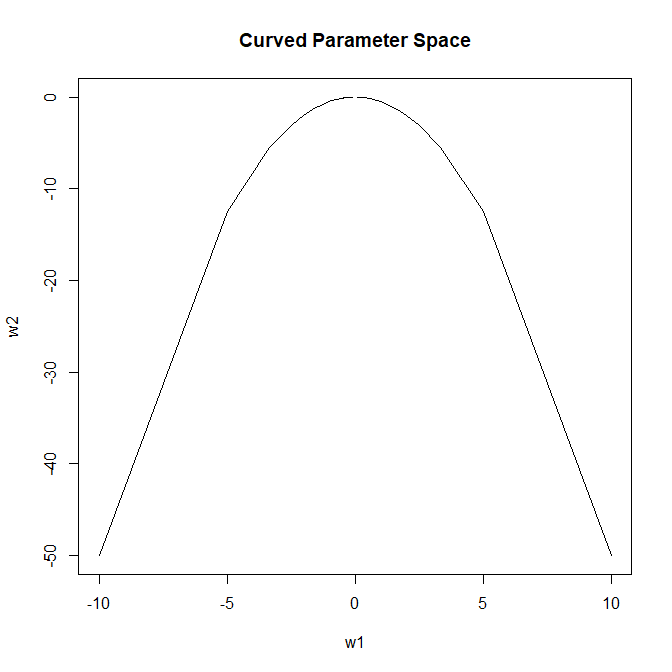
\includegraphics[width=0.8\textwidth]{7b.png}
      \end{center}
    \end{itemize}
  \end{itemize}
\end{problem}

\begin{problem}{8}
  Show that the following are not exponential families.
  \begin{enumerate}
    \item The uniform$(a, b)$ distributions.
    \item The (location-scale) logistic$(\mu, \beta)$ distributions. (See Example 3.10 in the notes.)
  \end{enumerate}
  \begin{enumerate}
    \item The pdf of uniform$(a, b)$ distributions is
    \[
      f(x) = \frac{1}{b-a}, \quad a < x < b.
    \]
    The support of $f$ is $(a,b)$, which depends on the parameters $a$ and $b$.
    Thus, the uniform$(a, b)$ distributions are not an exponential family.
    \item The pdf of logistic$(\mu, \beta)$ distributions is
    \[
      f(x) = \frac{e^{-\frac{x-\mu}{\beta}}}{\beta (1 + e^{-\frac{x-\mu}{\beta}})^2},
      \quad -\infty < x < \infty.
    \]
    \[
      \begin{aligned}
        f(x) &= \frac{e^{-\frac{x-\mu}{\beta}}}
        {\beta (1 + e^{-\frac{x-\mu}{\beta}})^2} \\
        &= \exp\left( -\frac{x-\mu}{\beta} - 
        \ln(\beta) - 2\ln(1 + e^{-\frac{x-\mu}{\beta}}) \right) \\
        &\text{Let } c(\mu, \beta) = \exp(-\ln(\beta)), h(x) = 1,\\
        &w_1(\mu, \beta) = \frac{1}{\beta}, w_2(\mu, \beta) = -\frac{1}{\beta},\\
        &t_1(x) = x, t_2(x) = \ln(1 + e^{-\frac{x-\mu}{\beta}})\\
        &\Rightarrow f(x) = c(\mu, \beta) h(x) e^{w_1(\mu, \beta) t_1(x) +
        w_2(\mu, \beta) t_2(x)}.
      \end{aligned}
    \]
    However, $t_2(x)$ depends on the parameters $\mu$ and $\beta$.
    Thus, the logistic$(\mu, \beta)$ distributions are not an exponential family.
  \end{enumerate}
\end{problem}
% --------------------------------------------------------------
%     You don't have to mess with anything below this line.
% --------------------------------------------------------------
\end{document}
